\documentclass[12pt]{amsart}
\usepackage{fullpage}
\usepackage{pbox}
\usepackage{graphicx}
\usepackage{booktabs} % Top and bottom rules for table
\usepackage{amsfonts, amsmath, amsthm, amssymb}
\usepackage{longtable,array,color,xcolor}
\usepackage[colorlinks = true,
            urlcolor  = blue]{hyperref}
\usepackage{verbatim}
\usepackage{enumerate}
\newcommand\narrowstyle{\SetTracking{encoding=*}{-50}\lsstyle}

\setlength{\parindent}{0pt}

\begin{document}
\flushright
Name:\underline{\hspace{5cm}}
\title{Math 320: Quiz 1}
\maketitle

\begin{enumerate}
\item (3 points) Review the code, and write down MATLAB's output.

\vspace{5mm}

\begin{verbatim} 
x = 3;
seq = [x];
while (x > 1)
    if (rem(x,2) == 0)  %rem(x,y) = remainder of x/y
        x = x/2;
    else
        x = 3*x + 1;
    end
    seq = [seq x];
end
disp(seq)

Output:
\end{verbatim}

\vspace{2cm}

\item (3 points) Draw (an approximation of) the plot output 
by the following MATLAB commands.

\begin{minipage}{.3\textwidth}
\begin{verbatim}
A = [1 2];
B = [1 1];
T = linspace(-pi,0,100);
X = 1.5 + cos(T);
Y = sin(T);
plot(A,B,'*',X,Y)
axis([-1,3,-2,2])
\end{verbatim}
\end{minipage}
\begin{minipage}{.6\textwidth}
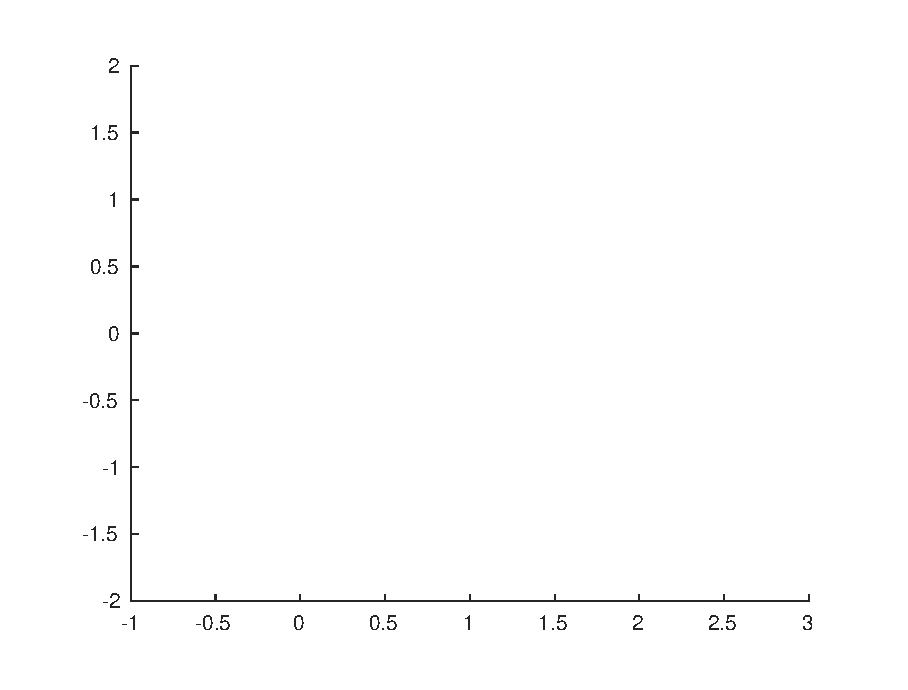
\includegraphics[scale=.7]{quiz1p2.eps}
\end{minipage}

\pagebreak

\item (4 points) Below is partial code for a function called 
{\tt pascal} that takes input {\tt n} and returns
the first {\tt n} rows of the Pascal triangle in an $n\times n$
square matrix with zeros above the diagonal.
One definition of Pascal's triangle is that $P_{i,1} = 1$
and $P_{i,j} = P_{i-1,j} + P_{i-1,j-1}$ for $j \neq 0$.

Please: \begin{enumerate} 
\item Comment the code where indicated by \% signs.
\item Fill in MATLAB code above each empty underline.
\item Evaluate {\tt pascal(5)}.

\vspace{1cm}

\begin{verbatim}
function P = pascal(n)
%

%

P = _____________ ; %Initializes P as an n x n Zero Matrix

for i=________

    P_______ = 1;
    
    for j=  __________  

        P(i,j) =  _________________ ;
    
    _____

____

____

\end{verbatim}
\hrulefill

{\tt pascal(5) = }

\end{enumerate}
\end{document}
